\documentclass[a4paper,11pt]{article}
\usepackage{amsmath,amsthm,amsfonts,amssymb,amscd,amstext,vmargin,graphics,graphicx,tabularx,multicol} 
\usepackage[francais]{babel}
\usepackage[utf8]{inputenc}  
\usepackage[T1]{fontenc} 
\usepackage{pstricks-add,tikz,tkz-tab,variations}
\usepackage[autolanguage,np]{numprint} 

\setmarginsrb{1.5cm}{0.5cm}{1cm}{0.5cm}{0cm}{0cm}{0cm}{0cm} %Gauche, haut, droite, haut
\newcounter{numexo}
\newcommand{\exo}[1]{\stepcounter{numexo}\noindent{\bf Exercice~\thenumexo} : \marginpar{\hfill /#1}}
\reversemarginpar


\newcounter{enumtabi}
\newcounter{enumtaba}
\newcommand{\q}{\stepcounter{enumtabi} \theenumtabi.  }
\newcommand{\qa}{\stepcounter{enumtaba} (\alph{enumtaba}) }
\newcommand{\initq}{\setcounter{enumtabi}{0}}
\newcommand{\initqa}{\setcounter{enumtaba}{0}}

\newcommand{\be}{\begin{enumerate}}
\newcommand{\ee}{\end{enumerate}}
\newcommand{\bi}{\begin{itemize}}
\newcommand{\ei}{\end{itemize}}
\newcommand{\bp}{\begin{pspicture*}}
\newcommand{\ep}{\end{pspicture*}}
\newcommand{\bt}{\begin{tabular}}
\newcommand{\et}{\end{tabular}}
\renewcommand{\tabularxcolumn}[1]{>{\centering}m{#1}} %(colonne m{} centrée, au lieu de p par défault) 
\newcommand{\tnl}{\tabularnewline}

\newcommand{\bmul}[1]{\begin{multicols}{#1}}
\newcommand{\emul}{\end{multicols}}

\newcommand{\trait}{\noindent \rule{\linewidth}{0.2mm}}
\newcommand{\hs}[1]{\hspace{#1}}
\newcommand{\vs}[1]{\vspace{#1}}

\newcommand{\N}{\mathbb{N}}
\newcommand{\Z}{\mathbb{Z}}
\newcommand{\R}{\mathbb{R}}
\newcommand{\C}{\mathbb{C}}
\newcommand{\Dcal}{\mathcal{D}}
\newcommand{\Ccal}{\mathcal{C}}
\newcommand{\mc}{\mathcal}

\newcommand{\vect}[1]{\overrightarrow{#1}}
\newcommand{\ds}{\displaystyle}
\newcommand{\eq}{\quad \Leftrightarrow \quad}
\newcommand{\vecti}{\vec{\imath}}
\newcommand{\vectj}{\vec{\jmath}}
\newcommand{\Oij}{(O;\vec{\imath}, \vec{\jmath})}
\newcommand{\OIJ}{(O;I,J)}


\newcommand{\reponse}[1][1]{%
\multido{}{#1}{\makebox[\linewidth]{\rule[0pt]{0pt}{20pt}\dotfill}
}}

\newcommand{\titre}[5] 
% #1: titre #2: haut gauche #3: bas gauche #4: haut droite #5: bas droite
{
\noindent #2 \hfill #4 \\
#3 \hfill #5

\vspace{-1.6cm}

\begin{center}\rule{6cm}{0.5mm}\end{center}
\vspace{0.2cm}
\begin{center}{\large{\textbf{#1}}}\end{center}
\begin{center}\rule{6cm}{0.5mm}\end{center}
}



\begin{document}
\pagestyle{empty}


\begin{center}
\textbf{ {\large Séance d'AP  : Trigonométrie}}
\end{center}

\vspace*{0.6cm}


\exo{}\\
En précisant le triangle rectangle utilisé,  écrire le quotient  de  deux longueurs égal à : 
\bmul{2}
\qa $cos$ $\widehat{GJI}$\\

\qa $sin$ $\widehat{IGH}$\\


\qa $tan$ $\widehat{HIG}$\\



\columnbreak

\begin{flushleft}
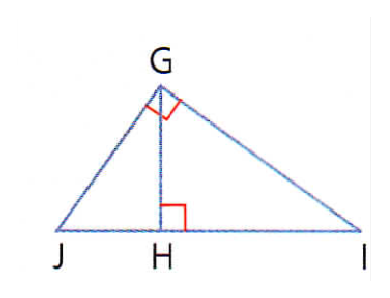
\includegraphics[scale=0.6]{trigo2.eps} 
\end{flushleft}

\emul

\vspace*{0.6cm}

\exo{} 


La distance entre le phare P du cap N'Doua et le ponton O de la tribu de Ouara est égale à environ 4,65 km. Un bateau B se trouve au large de ce ponton.\\
Le triangle OPB est rectangle en B et des visées ont permis d'établir que l'angle OPB est égal à 30\degre.

\begin{center}
 \includegraphics[scale=0.55]{trigo1.eps}
 \end{center} 

\q Montrer que la distance séparant le bateau B du ponton O est égale à 2 325 m.\\

\q Sachant que le bateau B se déplace à 15,5 km/h, déterminer
le temps (en minutes) qu'il lui faudra pour rejoindre le ponton
O.\\

\vspace*{0.6cm}


\exo{} 

Alexandre souhaite savoir à quelle distance il se trouve du Mont Saint Michel à l'aide d'un théodolite (appareil servant à mesurer des angles). \\
Il sait que le sommet du Mont est à 170 m d'altitude. \\
Son œil (O sur le dessin) étant situé à 1,60 m du sol, il obtient la mesure suivante : $ \widehat{SOH} = 25$\degre.\\

\begin{center}
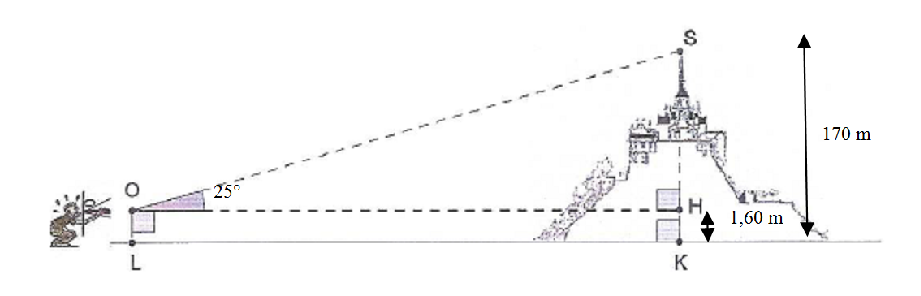
\includegraphics[scale=0.95]{trigo3.eps} 
\end{center}

A quelle distance LK du Mont se trouve-t-il ? (Donner une valeur approchée au mètre près). \\




\newpage

\vspace*{0.5cm}


\exo{}

Pour savoir si les feux de croisement de sa voiture sont réglés correctement, Pauline éclaire un mur vertical comme l'illustre le dessin suivant :

\begin{center}
\includegraphics[scale=0.6]{trigo6.eps} 
\end{center}

Pauline réalise le schéma ci-dessous (qui n'est pas à l'échelle) et relève les mesures suivantes : \\
PA = 0,65 m, AC = QP = 5 m et CK = 0,58 m.\\
P désigne le phare, assimilé à un point.

\begin{center}
\includegraphics[scale=0.85]{trigo7.eps} 
\end{center}

Pour que l'éclairage d'une voiture soit conforme, les constructeurs déterminent l'inclinaison du faisceau. Cette inclinaison correspond au rapport $\frac{\mathrm{QK}}{\mathrm{QP}}$. Elle est correcte si ce rapport est compris entre 0,01 et 0,015.\\

\initq \q Vérifier que les feux de croisement de Pauline sont réglés avec une inclinaison égale à 0,014.\\

\q Donner une mesure de l'angle $\widehat{\mathrm{QPK}}$ correspondant à l'inclinaison. On arrondira au dixième de degré.\\

\q Quelle est la distance AS d'éclairage de ses feux ? Arrondir le résultat au mètre près.\\

\vspace*{0.5cm}

\exo{}

Pour trouver la hauteur d'une éolienne, on a les renseignements suivants :\\

\noindent - Les points O, A et C sont alignés. \\
- Les points O, B et D sont alignés. \\
- Les angles $\widehat{OAB}$ et $\widehat{ACD}$ sont droits. \\
- OA = 1,1 m, AC = 20,9 m et AB = 1,5 m. \\

Le schéma n'est pas représenté en vraie grandeur. Le segment [CD] représente la hauteur de l'éolienne.\\

\begin{center}
\includegraphics[scale=0.6]{trigo5.eps} 
\end{center}


\initq \q Calculer la hauteur CD de l'éolienne. \\

\q Calculer la mesure de l'angle $\widehat{BOA}$ et donner le résultat au degré près. \\


\end{document}
